\documentclass{beamer}
\usepackage[utf8]{inputenc}
\usepackage{textpos}
\usepackage{hyperref}
\usepackage{minted}
\usepackage{etoolbox}
\AtBeginEnvironment{minted}{\fontsize{10}{10}\selectfont}

\usecolortheme{dove}

\title{Collaborating using Git and GitHub}
\author{Matthias Nilsson}
\institute{Chalmers University of Technology}
\date{June 12, 2015}

\logo{\includegraphics[height=1cm]{sysbio.jpg}\vspace{230pt}}

\definecolor{chalmersblue}{RGB}{0,0,102}
\setbeamercolor{footlinecolor}{fg=white,bg=chalmersblue}

\makeatother
\setbeamertemplate{footline}
{
  \leavevmode%
  \hbox{%
    \begin{beamercolorbox}[wd=\paperwidth,ht=8ex,dp=1ex,right]{footlinecolor}%
      \includegraphics[height=0.7cm]{cth.pdf}
      \hspace{1em}
    \end{beamercolorbox}%
  }
  \vskip0pt%
}
\setbeamertemplate{navigation symbols}{}

\newcommand{\fmtcmd}[1]{\mintinline{text}{#1}}

\begin{document}
{
\setbeamertemplate{logo}{\includegraphics[height=2cm]{sysbio.jpg}\vspace{200pt}}
\begin{frame}
\maketitle
\end{frame}
}

\begin{frame}{}
  Before we start:

  \small
  \begin{enumerate}
    \item Run \fmtcmd{git config --global merge.ff only}
    \item Create a new directory for today's workshop
    \item Go to \url{https://github.com/SysBioChalmers/git_collaboration} and fork it
    \item Run \scriptsize\fmtcmd{git clone https://github.com/SysBioChalmers/git_collaboration.git}
  \end{enumerate}
\end{frame}

\begin{frame}{Today's goals}
  \begin{itemize}
  \item Know how to work with other in the same repo
  \item Know how to handle (Git) conflicts
  \item Know how to create pull requests
  \end{itemize}
\end{frame}

\begin{frame}{}
  \center
  \Huge But first...
\end{frame}

\begin{frame}{}
  \center
  \Huge Ignoring files
\end{frame}

\begin{frame}{Ignoring files}
  \center
  \Huge We want to track our work
  \pause

  \huge But we don't necessarily want to track \emph{all} the files
\end{frame}

\begin{frame}{Ignoring files}
  \center
  \huge In general, we are not interested in tracking the history of
  \emph{generated} files
  \pause

  \Large (E.g. the PDF that is produced when we compile our \LaTeX\ 
  presentation)
\end{frame}

\begin{frame}{Ignoring files}
  \center
  \Huge We can tell Git to ignore files by adding a
  \fmtcmd{.gitignore} file to our repository
\end{frame}

\begin{frame}[fragile]{Ignoring files}
  \begin{minted}{text}
    $ cat .gitignore
    *.pdf
    *.aux
    *.log
    *.nav
    *.out
    *.snm
    *.toc
    *.vrb
    _minted*
  \end{minted}
\end{frame}

\begin{frame}{Ignoring files}
  \fmtcmd{.gitignore}:
  \begin{itemize}
    \item One line per \emph{pattern}
    \item Wildcards (\fmtcmd{*}) are allowed
  \end{itemize}
\end{frame}

\begin{frame}{}
  \center
  \Huge And now...
\end{frame}

\begin{frame}{}
  \center
  \Huge Getting new changes
\end{frame}

\begin{frame}{Getting new changes}
  \center
  \Huge To update our local repository, we use \fmtcmd{git
    pull}
\end{frame}

\begin{frame}{}
  \center
  \Huge Exercise 1: Updating a read-only repo
\end{frame}

\begin{frame}{Exercise 1}
  \center
  \LARGE For this exercise we will use the \fmtcmd{git_collaboration}
  repo that you cloned at the start of the workshop
\end{frame}

\begin{frame}{Exercise 1}
  \center
  \Huge Has everyone cloned the SysBioChalmers
  \fmtcmd{git_collaboration} repo?
\end{frame}

\begin{frame}[fragile]{Exercise 1}
  Outcome:

  \begin{minted}{text}
    $ git status
    On branch master
    Your branch is up-to-date with 'origin/master'.
    nothing to commit, working directory clean
  \end{minted}
\end{frame}

\begin{frame}[fragile]{Exercise 1}
  Commands:

  \begin{minted}{text}
    $ git fetch --all
    $ git status
    $ git pull
  \end{minted}
\end{frame}

\begin{frame}{}
  \center
  \Huge Exercise 2: Working together in the same repo
\end{frame}

\begin{frame}{Exercise 2}
  What we will go through:

  \begin{enumerate}
    \item Preparation
    \item Diverging branches
    \item Conflicts
  \end{enumerate}
\end{frame}

\begin{frame}{Exercise 2}
  \center
  \Huge Preparation
\end{frame}

\begin{frame}{Exercise 2 - Preparation}
  \center
  \LARGE We will simulate some common scenarios and go through how to
  solve each one
\end{frame}

\begin{frame}{Exercise 2 - Preparation}
  \center
  \Large Make three different clones of your own repo:
  \fmtcmd{git_collaboration1}, \fmtcmd{git_collaboration2}, and
  \fmtcmd{git_collaboration3}
  \pause

  \Large (Make sure you use the SSH clone URL and that you use
  \emph{your} repo, since you need write permissions)
\end{frame}

\begin{frame}[fragile]{Exercise 2 - Preparation}
  Go to \fmtcmd{git_collaboration1}, open up \fmtcmd{README.md}, add
  the following to the end, and commit:

  \begin{minted}{text}
    # Another section
    With some text
  \end{minted}
\end{frame}

\begin{frame}[fragile]{Exercise 2 - Preparation}
  Add the following to the end and commit:
  \begin{minted}{text}
    # Yet another section
    With some more text
  \end{minted}
\end{frame}

\begin{frame}[fragile]{Exercise 2 - Preparation}
  \fmtcmd{README.md} should look like this now:

  \begin{minted}{text}
    # git_collaboration
    Training repo for Git collaboration workshop

    # Another section
    With some text

    # Yet another section
    With some more text
  \end{minted}
\end{frame}

\begin{frame}{Exercise 2 - Preparation}
  \center
  \huge Push your changes
\end{frame}

\begin{frame}{Exercise 2}
  \center
  \Huge Diverging branches
\end{frame}

\begin{frame}{Exercise 2 - Diverging branches}
  \center
  \Large Branches are said to \emph{diverge} when they have a common
  root and one or more commits that do not exist in the other branch
\end{frame}

\begin{frame}{Exercise 2 - Diverging branches}
  \center
  \Large Common scenario: Our collaborator has pushed changes to
  GitHub and we have commits locally that are not pushed yet
\end{frame}

\begin{frame}{Exercise 2 - Diverging branches}
  \center
  \huge This is what the branch looks like:

  \vspace{0.3cm}
  \includegraphics[height=2cm]{pre_rebase.pdf}
  \pause

  \LARGE \fmtcmd{D} is our local commit, \fmtcmd{E} and \fmtcmd{F} are
  new commits on origin (GitHub)
\end{frame}

\begin{frame}{Exercise 2 - Diverging branches}
  \begin{enumerate}
    \item Go to \fmtcmd{git_collaboration2}
    \item Create a \emph{new} file, add it, and commit
    \item Run \fmtcmd{git fetch --all}
    \item Run \fmtcmd{git status}
  \end{enumerate}
\end{frame}

\begin{frame}{Exercise 2 - Diverging branches}
  \center
  \Huge Try pulling in the changes with \fmtcmd{git pull}
  \pause

  \vspace{0.5cm}
  \Huge Git will refuse
\end{frame}

\begin{frame}{Exercise 2 - Diverging branches}
  \center
  \Huge Try pushing your changes with \fmtcmd{git push}
  \pause

  \vspace{0.5cm}
  \Huge Git will refuse
\end{frame}

\begin{frame}{Exercise 2 - Diverging branches}
  \center
  \Huge Git will avoid overwriting commits
  \pause

  \LARGE This means that we will have to instruct Git how to handle
  the divergence
\end{frame}

\begin{frame}{Exercise 2 - Diverging brances}
  \center
  \huge We want to go from this:
  \includegraphics[width=6cm]{pre_rebase.pdf}
  \pause

  \huge To this:
  \vspace{0.1cm}

  \includegraphics[width=7cm]{post_rebase.pdf}
\end{frame}

\begin{frame}{Exercise 2 - Diverging branches}
  \center
  \LARGE ``Take the commits on origin and add my commits after them''
\end{frame}

\begin{frame}{Exercise 2 - Diverging branches}
  \center
  \Huge \fmtcmd{git pull --rebase}
\end{frame}

\begin{frame}{Exercise 2 - Diverging branches}
  Check what the outcome was:

  \begin{itemize}
    \item Run \fmtcmd{git log}
    \item Run \fmtcmd{git fetch --all}
    \item Run \fmtcmd{git status}
  \end{itemize}
\end{frame}

\begin{frame}{Exercise 2 - Diverging branches}
  \center
  \Huge We can now push our changes
\end{frame}

\begin{frame}{Exercise 2}
  \center
  \Huge Conflicts
\end{frame}

\begin{frame}{Exercise 2 - Conflicts}
  \center
  \huge A \emph{conflict} is when there are two different changes in
  the same place
  \pause

  \LARGE And we try to combine these changes
\end{frame}

\begin{frame}{Exercise 2 - Conflicts}
  \center
  \Huge Example: When two people change the same line but in different ways
\end{frame}

\begin{frame}{Exercise 2 - Conflicts}
  \center
  \Huge Git leaves it up to us to resolve these situations
\end{frame}

\begin{frame}{Exercise 2 - Conflicts}
  \center
  \huge Go to \fmtcmd{git_collaboration3}
\end{frame}

\begin{frame}[fragile]{Exercise 2 - Conflicts}
  Open up \fmtcmd{README.md} and edit it to make it look like this:

  \begin{minted}{text}
    # git_collaboration
    Training repo for Git collaboration workshop

    # My favorite color
    Black
  \end{minted}
\end{frame}

\begin{frame}{Exercise 2 - Conflicts}
  \center
  \huge Commit your changes and run \fmtcmd{git fetch --all}
\end{frame}

\begin{frame}{Exercise 2 - Conflicts}
  \center
  \huge \fmtcmd{git status} tells us that our local master has diverged from origin
  \pause

  \LARGE Run \fmtcmd{git pull --rebase} to solve this
\end{frame}

\begin{frame}[fragile]{Exercise 2 - Conflicts}
  \begin{minted}{text}
    $ git pull --rebase
    ...
    Auto-merging README.md
    CONFLICT (content): Merge conflict in README.md
    ...
  \end{minted}
\end{frame}

\begin{frame}[fragile]{Exercise 2 - Conflicts}
  \begin{minted}[fontsize=\scriptsize]{text}
    $ git status
    rebase in progress; onto xxxxxxx
    You are currently rebasing branch 'master' on 'xxxxxxx'.
    (fix conflicts and then run "git rebase --continue")
    (use "git rebase --skip" to skip this patch)
    (use "git rebase --abort" to check out the original branch)

    Unmerged paths:
    (use "git reset HEAD <file>..." to unstage)
    (use "git add <file>..." to mark resolution)

          both modified:   README.md
  \end{minted}
\end{frame}

\begin{frame}{Exercise 2 - Conflicts}
  Workflow:

  \begin{enumerate}
    \item Resolve the conflict
    \item Run \fmtcmd{git add} on the file(s)
    \item Run \fmtcmd{git rebase --continue} to proceed
  \end{enumerate}
\end{frame}

\begin{frame}[fragile]{Exercise 2 - Conflicts}
  Open up \fmtcmd{README.md} in an editor. It should look something like this:

  \begin{minted}{text}
    # git_collaboration
    Training repo for Git collaboration workshop

    <<<<<<< HEAD
    # Another section
    With some text

    # Yet another section
    With some more text
    =======
    # My favorite color
    Black

    >>>>>>> add color section
  \end{minted}
\end{frame}

\begin{frame}{Exercise 2 - Conflicts}
  \center
  \huge Git shows us the two different versions and leaves it up to us
  to decide what the ``right'' version is
\end{frame}

\begin{frame}[fragile]{Exercise 2 - Conflicts}
  \Large Replace the marked region with the right version:
  \vspace{0.5cm}

  \begin{tabular}{ p{0.3\textwidth} r p{0.3\textwidth} }
    \begin{minipage}{0.3\textwidth}
    \begin{minted}[fontsize=\tiny]{text}
      # git_collaboration
      Training repo for Git collaboration workshop

      <<<<<<< HEAD
      # Another section
      With some text

      # Yet another section
      With some more text
      =======
      # My favorite color
      Black

      >>>>>>> add color section
    \end{minted}
    \end{minipage}
    &
      \hspace{1cm}
      $ \rightarrow $
    &
    \begin{minipage}{0.3\textwidth}
    \begin{minted}[fontsize=\tiny]{text}
      # git_collaboration
      Training repo for Git collaboration workshop

      # Another section
      With some text

      # Yet another section
      With some more text

      # My favorite color
      Black

    \end{minted}
    \end{minipage}
    \\
  \end{tabular}
\end{frame}

\begin{frame}{Exercise 2 - Conflicts}
  \center

  \huge Tell Git that the conflict is resolved by using \fmtcmd{git add}
\end{frame}

\begin{frame}{Exercise 2 - Conflicts}
  \center
  \huge Continue the process by running \fmtcmd{git rebase
    --continue}
\end{frame}

\begin{frame}{Exercise 2 - Conflicts}
  \center
  \huge Run \fmtcmd{git log -p} to look at the changes as well as the commit messages
\end{frame}

\begin{frame}{Exercise 2 - Conflicts}
  \center
  \huge We can now push our changes
\end{frame}

\begin{frame}{}
  \center
  \Huge Working with feature branches
\end{frame}

\begin{frame}{Feature branches}
  \center
  \huge Coordinating multiple people working in the same branch is a challenge
  \pause

  \Large (E.g. since we must keep our local repo up to date to be able to push)
\end{frame}

\begin{frame}{Feature branches}
  \center
  \Huge We can simplify by separating the work into different branches
\end{frame}

\begin{frame}{Feature branches}
  \center
  \huge Example: When writing a paper, we can have one branch for each section
  \pause

  \LARGE This allows us to work (more) undisturbed
\end{frame}

\begin{frame}{}
  \center
  \Huge Collaborating using pull requests
\end{frame}

\begin{frame}{Pull requests}
  \center
  \huge Pull requests are used to contribute to a project on GitHub
\end{frame}

\begin{frame}{Pull requests}
  Workflow:

  \begin{enumerate}
    \item Create a feature branch in your forked repo (make sure to push
      the branch to GitHub)
    \item Make your changes
    \item Commit and push
    \item Submit a pull request to let the maintainer know about your
      work
  \end{enumerate}
\end{frame}

\begin{frame}{Pull requests}
  Creating a pull request:

  \begin{enumerate}
    \item Go to \fmtcmd{https://github.com/<your GitHub ID>/git_collaboration}
    \item Click on ``Pull requests'' in the menu on the right
    \item Click on ``New pull request''
  \end{enumerate}
\end{frame}

\begin{frame}{Pull requests}
  \center
  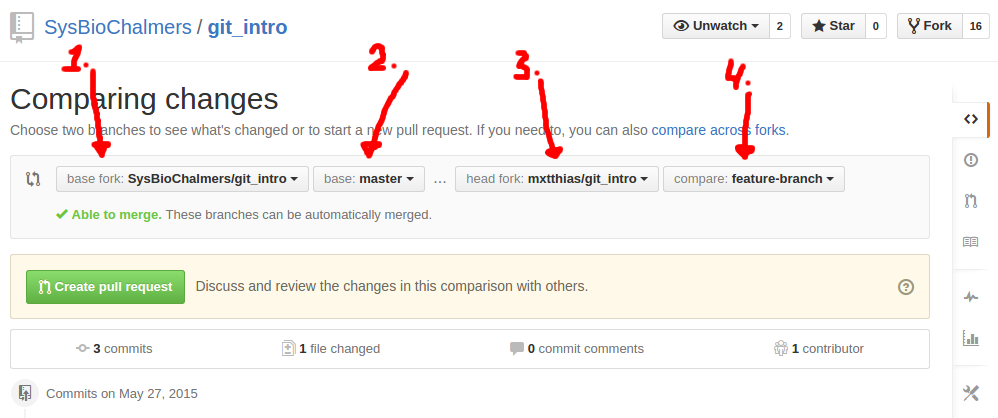
\includegraphics[height=3cm]{comparing_changes.png}

  1. Target repo, 2. Target branch, 3. Source repo, 4. Source branch
\end{frame}

\begin{frame}{Pull requests}
  \center
  \Large \url{https://help.github.com/articles/using-pull-requests/}
\end{frame}

\begin{frame}{Pull requests}
  Homework:

  \begin{enumerate}
    \item Add a line with your favorite color to \fmtcmd{README.md} in
      \fmtcmd{<your GitHub ID>/git_collaboration}
    \item Create a pull request to \fmtcmd{SysBioChalmers/git_collaboration}
  \end{enumerate}
\end{frame}

\begin{frame}{}
  \center
  \Huge Questions?
\end{frame}

\end{document}